% 电阻 欧姆定律
% 电阻|导体|电流|电压|欧姆定律

\pentry{电流\upref{I}, 电压\upref{Voltag}}

\textbf{欧姆定律}为
\begin{equation}
U = IR
\end{equation}
其中 $U$ 是\textbf{电阻器}\footnote{在可能混淆的情况下, 为了区分 “电阻” 这个词作为电路元件和作为物理量, 我们把前者叫做 “电阻器”, 后者叫做 “电阻”.}两端的电压, $I$ 是流经电阻器的电流, $R$ 是电阻器的电阻.

作为一个理想模型, 柱形(例如长方体, 圆柱体)电阻器的电阻为
\begin{equation}
R = \frac{\varrho L}{S} 
\end{equation}
其中 $S$ 为电阻的横截面积, $L$ 为电阻的长度, $\varrho$ 为材料的\textbf{电阻率}. 电阻率体现了材料电阻能力, 和材料性质有关, 也可能会随温度,压强,光照(例如光敏电阻),等环境因素变化. 我们也通常把电阻率的倒数 $1/\varrho$ 叫做\textbf{电导率}.

微观形式的欧姆定律为
\begin{equation}
\bvec E = \varrho\bvec j
\end{equation}
这个公式告诉我们, 电阻材料中某点的电流密度与电场成正比.

\subsection{电阻的简单模型}
\begin{figure}[ht]
\centering
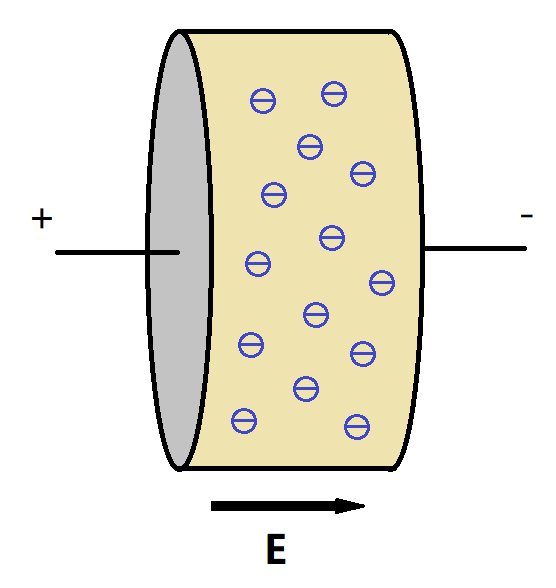
\includegraphics[width=4cm]{./figures/Resist_1.png}
\caption{简单的电阻模型: 一个平行板电容器中均匀填充导电介质} \label{Resist_fig1}
\end{figure}

我们这里用一个简单的经典力学模型推导上文中的概念和公式, 但严格来说, 这个推导需要使用量子力学和半导体理论. 假设一个平行板电容器中间有某种均匀的导电材料, 该材料中自由电子的电荷密度为 $-\rho$ ($\rho > 0$) 为定值, 每个电子受到的阻力与电子速度成正比, 比例常数 $\alpha > 0$. 即
\begin{equation}
\bvec f = -\alpha \bvec v
\end{equation}
当我们在电容器两板上施加电压时, 内部会产生匀强电场, 使电子受到电场力
\begin{equation}
\bvec F = -e\bvec E
\end{equation}
电子在该电场力下加速(由于电子质量很小, 加速过程很快, 可以假设是一瞬间完成的), 直到阻力等于电场力时加速停止, 进行匀速运动. 于是有
\begin{equation}
-e\bvec E - \alpha \bvec v = \bvec 0 \Rightarrow \bvec v = -\frac{e}{\alpha}\bvec E
\end{equation}
所以电阻内电流密度大小为
\begin{equation}\label{Resist_eq4}
\bvec j = -\rho \bvec v = \frac{e\rho}{\alpha}\bvec E
\end{equation}
电流大小为
\begin{equation}
I = jS = \frac{\rho EeS}{\alpha}
\end{equation}
电阻中的电场大小可以由两端电压表示为
\begin{equation}
E = \frac UL
\end{equation}
带入上式得
\begin{equation}\label{Resist_eq3}
U = I \frac{\alpha L}{\rho eS}
\end{equation}
我们定义\textbf{电阻率}为
\begin{equation}\label{Resist_eq1}
\varrho = \frac{\alpha}{\rho e}
\end{equation}
然后再根据电阻率定义\textbf{电阻}为
\begin{equation}\label{Resist_eq2}
R = \frac{\varrho L}{S}
\end{equation}
可见它与长度 $L$ 成正比, 与横截面成反比. 将\autoref{Resist_eq1} 带入\autoref{Resist_eq2} 再带入\autoref{Resist_eq3}, 可得\textbf{欧姆定律}
\begin{equation}
U = IR
\end{equation}
\autoref{Resist_eq4} 也可以使用电阻率记为
\begin{equation}
\bvec E = \varrho\bvec j
\end{equation}
这相当于欧姆定律的微观形式.
